\documentclass[a4paper]{jpconf}
\usepackage{graphicx}

\usepackage{tikz}

\begin{document}
\title{Modelling dynamic processes in a nuclear reactor by state change modal method}

\author{A V Avvakumov$^1$, V F Strizhov$^2$, P N Vabishchevich$^{2,3}$ and A O Vasilev$^3$}

\address{$^1$ National Research Center Kurchatov Institute, Moscow, Russia}
\address{$^2$ Nuclear Safety Institute of RAS, Moscow, Russia}
\address{$^3$ North-Eastern Federal University, Yakutsk, Russia}

\ead{haska87@gmail.com}

\begin{abstract}
Modelling of dynamic processes in nuclear reactors is carried out, mainly, on
the basis of the multigroup diffusion approximation for the neutron flux. 
The basic model includes a multidimensional set of coupled parabolic equations and
ordinary differential equations.
Dynamic processes are modelled by a successive
change of the reactor states, which are characterized by given coefficients of the equations. 
It is considered that the transition from one state to another occurs instantaneously.
In the modal method the approximate solution is represented as eigenfunction expansion. 
The numerical-analytical method is based on the use of dominant time-eigenvalues of
a multigroup diffusion model taking into account delayed neutrons. 
%For each reactor state the eigenvalues and eigenfunctions of the $\alpha$-eigenvalue problem are calculated in advance.
%This provides very fast calculations in real-time scale.
%Numerical simulations of the dynamic process were performed in the framework of the
%two-group approximation for the VVER-1000 reactor test model. 
%The last is characterized by the fact that some eigenvalues are complex.
%The dynamic model includes two reactor states, namely the regular regime of the supercritical state with further transition to the subcritical state.
%The results of the dynamic process simulation demonstrate the acceptable accuracy in calculation of neutron power and delayed neutrons source in comparison with the direct dynamic calculation.
\end{abstract}

\section{Introduction}
These guidelines show how to prepare articles for publication in \jpcs\ using \LaTeX\ so they can be published quickly and accurately. Articles will be refereed by the \corg s but the accepted PDF will be published with no editing, proofreading or changes to layout. It is, therefore, the author's responsibility to ensure that the content and layout are correct.  This document has been prepared using \cls\ so serves as a sample document. The class file and accompanying documentation are available from \verb"http://jpcs.iop.org".

\section{Problem statement}

The neutron flux is modelled in multigroup diffusion approximation taking into account delayed neutrons. The neutron dynamics is considered in the bounded convex three-dimensional area with corresponding initial and
boundary conditions. We will use the following simplified description of the dynamic processes in a nuclear reactor. In selected time interval, the non-stationary neutron flux is determined by the nuclear reactor state. The state of the reactor is characterized by the constant coefficients of the system of multigroup diffusion equations. Dynamic processes in a nuclear reactor can be considered as an instantaneous change of states (see  Fig.\ref{fig:1}).
\begin{figure}[] 
  \begin{center}
\vspace{5mm} 
    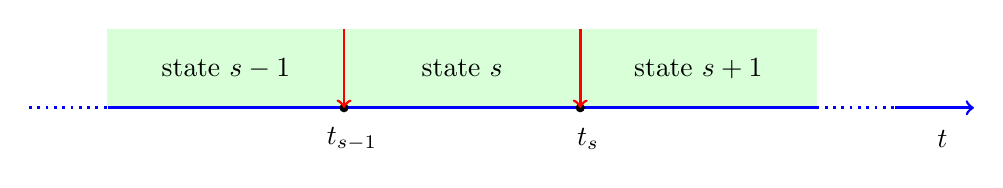
\begin{tikzpicture}
      \filldraw [color=green!15] (0,0) rectangle +(9,1);
      \draw [dotted, line width=1, color=blue] (-1,0) -- (0,0);
      \draw [line width=1, color=blue] (0,0) -- (9,0);
      \draw [dotted, line width=1, color=blue] (9,0) -- (10,0);
      \draw [->, line width=1, color=blue] (10,0) -- (11,0);
      \filldraw [black] (3,0) circle (0.05);
      \filldraw [black] (6,0) circle (0.05);
      \draw  (1.5,0.5) node {state $s-1$};  
      \draw  (4.5,0.5) node {state $s$};  
      \draw  (7.5,0.5) node {state $s+1$};  
      \draw  (3.1,-0.4) node {$t_{s-1}$}; 
      \draw  (6.1,-0.4) node {$t_{s}$}; 
      \draw  (10.6,-0.4) node {$t$}; 
      \draw [->, line width=1, color=red] (3,1) -- (3,0);
      \draw [->, line width=1, color=red] (6,1) -- (6,0);
    \end{tikzpicture}
    \caption{State change scheme.} 
   \label{fig:1}
  \end{center}
\end{figure}

Simulation of the dynamic behavior of the reactor consists in solving the sequence of subtasks for the individual states of the reactor. The initial condition for the state $s$ (at $t = t_{s-1}$) is the final state of the reactor for the state $s-1$.

An approximate description of the non-stationary process at a separate stage is based on modal approximation. An approximate solution is sought in the form of an expansion in eigenfunctions time-eigenvalue, $\alpha$-eigenvalue problem. Finite-element approximation in space is used. 

The modal approximation corresponds to the representation of the approximate solution of problem as a sum of dominant eigenfunctions with corresponding coefficients. Each eigenfunction is the solution of the  $\alpha$-eigenvalue problem.
To find the coefficients, a system of linear equations is solved. The state change modal method is based on the following calculating scheme.
\begin{description}
 \item[Off-line calculation.] Calculation of the coefficients of the mathematical model of the multigroup diffusion approximation for the isolated reactor states, which is performed in advance. The status passport also includes calculated dominant eigenvalues and eigenfunctions of the  $\alpha$-eigenvalue problem. 
These data can be supplemented by dominant eigenvalues and eigenvalues of the conjugate eigenvalue problem.
 \item[On-line calculation.] Real-time modeling is carried out on the basis of the modal solution of the problem.
The coefficients in the representation  are calculated from the initial condition.    
\end{description}  
 
A test problem for a VVER-1000 reactor without a reflector is considered in the two-dimensional approximation.
The dominant eigenvalues were calculated (some of them are complex). In our example, the main eigenvalue is negative and therefore the major harmonic will increase, and all others will fade. This demonstrates the regular mode of the reactor operation. The value $\alpha = \lambda_1^{(\alpha)}$ itself determines the neutron flux amplitude and is directly related to the reactor period in the regular regime.

The problem of simulation of reactor dynamic processes is considered on the basis of multigroup neutron diffusion equations taken into account delayed neutrons.
The modal approximation is used: an approximate solution is represented as an expansion on few dominant eigenfunctions of the $\alpha$-eigenvalue spectral problem.

Numerical simulation of reactor non-stationary processes is carried out on the basis of a successive change in the states of the reactor. These states are characterized by a set of constant parameters to describe the multigroup neutron flux behavior.
The state change modal method was developed. The phase, which described fast transition to the approximate solution, is selected as a set of dominant modes. At a slow phase of the reactor dynamics, the solution is based on the evolution of dominant modes.

The computational implementation of the state change modal method is based on the previously calculated (of-line calculation) eigenfunctions and eigenvalues of the  $\alpha$-eigenvalue spectral problem. Fast determination of dominant modes and calculation of the reactor neutron flux at selected times are based on on-line calculation.
The classical Lagrange finite elements $p=1,2,3$ are used for the spatial approximation. 
Accuracy control is performed using condensed grids. Spectral problems are solved numerically using well-developed free software SLEPc.

Test calculations are made in two-dimensional analysis using a two-group diffusion approximation. Calculations of dominant modes for a reactor supercritical state are performed. The major mode solution, which determines the reactor regular regime, is used as the initial condition for transition to the subcritical state. The modeling of the reactor dynamics change as a transfer from one state to another state is carried out for two variants. The first of them (symmetric perturbation) is due to the uniform change in the absorbing material properties. The second variant (asymmetric perturbation) deals with a non-uniform change in the absorbing material properties (in two halves over the reactor cross-section).

Comparison of the calculational results obtained by using two methods (one based on modal approximation and another based on the full dynamics calculation) shows the acceptable accuracy in calculation of neutron power and delayed neutrons source for the VVER-1000 test problem. 

\section*{References}
\begin{thebibliography}{9}
\bibitem{iopartnum} IOP Publishing is to grateful Mark A Caprio, Center for Theoretical Physics, Yale University, for permission to include the {\tt iopart-num} \BibTeX package (version 2.0, December 21, 2006) with  this documentation. Updates and new releases of {\tt iopart-num} can be found on \verb"www.ctan.org" (CTAN). 
\end{thebibliography}

\end{document}


